\documentclass[12pt]{amsart}
\usepackage[fullpage]{geometry}
\usepackage{fullpage}
\usepackage{pbox}
\usepackage{graphicx}
\usepackage{booktabs} % Top and bottom rules for table
\usepackage{amsfonts, amsmath, amsthm, amssymb}
\usepackage{longtable,array,color,xcolor}
\usepackage[colorlinks = true,
            urlcolor  = blue]{hyperref}
\usepackage{verbatim}
\usepackage{enumerate}
\newcommand\narrowstyle{\SetTracking{encoding=*}{-50}\lsstyle}
\newcommand{\RR}{\mathbb{R}}

\setlength{\parindent}{0pt}

\begin{document}

\title{Math 320: Homework 6}
Due: November 9, 2016
\maketitle

Please read through chapters 11, 12.1, and 13 in the textbook.
Answer the following questions. Please submit all code
and output with brief descriptions of what you are doing.

\vspace{5mm}

\begin{enumerate}

\item Section 11.2 discusses various norms on matrices.
In class, we reviewed three properties of any matrix norm $\rho$:
\begin{enumerate}
\item $\rho(a M) = a \rho(M)$ for scalar $a$ and matrix $M$.
\item $\rho( M + N) \leq \rho(M) + \rho(N)$ for $M,N$ matrices.
\item $\rho(M) = 0$ only if $M$ is the zero matrix.
\end{enumerate}
Prove that these properties are satisfied for 1) the column-sum
norm, and 2) the spectral norm. \\ 
{\bf Hint:} for the spectral norm,
use the induced norm definition: 
$||M||_2 = \sup(||Mx||_2 /||x||_2)$, where the
norm on the right-hand side is the Euclidean norm on vectors.

\vspace{5mm}

Recall that the column-sum norm is given by 
$||M||_1 = \max_{j} \sum_{i = 1}^n |M_{ij}|$. We prove
each of the desired properties:

\begin{enumerate}
\item $|| a M ||_1 = |a| || M||_{1}$ for scalar $a$ and matrix $M$.

$|| a M ||_1 = \max_{j} \sum_{i = 1}^n |aM_{ij}| = \max_{j} \sum_{i = 1}^n |a||M_{ij}| = |a| \max_{j} \sum_{i = 1}^n | M_{ij}| = |a| ||M||_{1}$.


\item $|| M + N ||_1 \leq ||M||_1 + ||N||_1$ for $M,N$ matrices.

$||M+N||_1 = \max_{j} \sum_{i = 1}^n | M_{ij} + N_{ij}|$. By the triangle
inequality for real numbers, $|M_{ij} + N_{ij}| \leq |M_{ij}| + |N_{ij}|$.

Therefore, 
\[ \max_{j} \sum_{i = 1}^n | M_{ij} + N_{ij}| \leq
\max_{j} \sum_{i = 1}^n |M_{ij} + N_{ij}| \leq \max_j \left(\sum_{i = 1}^n |M_{ij}|
+ \sum_{i = 1}^n |N_{ij}|\right).\]
 If we independently maximize over each
sum, it will be at least as large as maximizing them together; so:

\[ \max_j \left(\sum_{i = 1}^n |M_{ij}|
+ \sum_{i = 1}^n |N_{ij}|\right) \leq 
\max_j \left(\sum_{i = 1}^n |M_{ij}|\right)
+ \max_j\left( \sum_{i = 1}^n |N_{ij}|\right) = ||M||_1 + ||N||_1.
\]

\item $||M||_1 = 0$ only if $M$ is the zero matrix.

Suppose that $M$ is not the zero matrix. Then some entry
of the matrix is nonzero; call this entry $M_{rs}$. Then,
$||M||_1 = \max_j \sum_{i = 1}^n |M_{ij}|$ must be {\em at least} 
as large as $\sum_{i = 1}^n |M_{is}| \geq |M_{rs}| \neq 0$.
\end{enumerate}


We now do the same for the spectral norm:

\begin{enumerate}
\item $||a M||_2= |a| ||M||_2$ for scalar $a$ and matrix $M$.

Recall that $||M||_2 = \sup_x(||Mx||_2 /||x||_2)$, so:
\[||a M||_2= \sup_x(||aMx||_2 /||x||_2) = \sup(|a| ||Mx||_2 /||x||_2)
|a| \sup(||Mx||_2 /||x||_2) = |a| ||M||_2.
\]

\item $||M + N||_2 \leq ||M||_2 $ for $M,N$ matrices.  

\[||M+ N||_2= \sup_x(||(M+N)x||_2 /||x||_2) = \sup_x(||Mx + Nx||_2 /||x||_2) \text{  (by linearity)}\]
\[ \leq \sup_x(||Mx||_2 + ||Nx||_2 /||x||_2) \text{ (by triangle inequality for $2$-norm)}
\]
\[ = \sup_x \left(\dfrac{||Mx||_2}{||x||_2} + \dfrac{||Nx||_2}{||x||_2} \right) \leq 
\sup_x \left(\dfrac{||Mx||_2}{||x||_2} \right) +\sup_x\left( \dfrac{||Nx||_2}{||x||_2} \right) = ||M||_2 + ||N||_2
\]
\item $||M||_2 = 0$ only if $M$ is the zero matrix.
Suppose that $M$ is not the zero matrix. Then $M_{rs} \neq 0$ for some $r,s$.
Take $x = e_s$, i.e. the vector which is one in the $s$-th coordinate and
zero elsewhere. Then $Mx = M_{rs} e_r +$ an orthogonal component. For this vector
$||Mx||_2/||x||_2 \geq |M_{rs}|$; therefore, the supremum over all $x$ is at
least this large. This means that $||M||_2 > 0$.
\end{enumerate}

\vfill
\pagebreak


\item Problem 11.9.

\vspace{5mm}

\begin{enumerate}
\item Determine the condition number based on the row-sum
norm for the case where $x_1 = 4, x_2 = 2, x_3 = 7$.

\vspace{1cm}

For this version, we need to compute explicitly by finding the
row-sum norm of the matrix and its inverse.

In this case, the matrix and its inverse (computed using Gaussian
elimination) are:

\[
\left[\begin{array}{ccc}
16 & 4 & 1 \\
4 & 2 & 1 \\
49 & 7 & 1 \\
\end{array} \right] \hspace{2cm}
\left[\begin{array}{ccc}
-1/6 & 1/10 & 1/15 \\
3/2 & -11/10 & -2/5 \\
-7/3 & 14/5 & 8/15 \\
\end{array} \right]
\]
In the first matrix, the third row is largest with sum $57$; in the
second matrix, the third row is largest with 
$\sum |A_{3j}| = 17/3 \approx 5.667$. So, the condition number
 based on row-sum norm is $57 \times 17/3 = 323$.

\vspace{5mm}

\item Use MATLAB to compute the spectral and Frobenius condition numbers.

\vspace{1cm}
Here, we use the MATLAB commands written below:
\begin{verbatim}
N = [16 4 1; 4 2 1; 49 7 1];
cond(N,'fro') %Condition number based on Frobenius norm
cond(N,2)     %Condition number based on spectral norm (or induced 2-norm)
\end{verbatim}
The results are: Frobenius condition number 217.4843 and spectral
condition number 216.1294.
\end{enumerate}

\vfill
\pagebreak








\item Problem 12.2. You may use the textbook implementation of
Gauss-Seidel, but add a subroutine that at each iteration, plots the
first two coordinates of the approximation.
Display the plots for part (a) and part (b).

\vspace{5mm}

The following code is adapted from the Gauss-Seidel implementation
in the textbook. The two primary changes are the inclusion of
relaxation using the {\tt lambda} parameter and the plot command
in the loop.

\begin{verbatim}
function x = GaussSeidel(A,b,lambda,es,maxit)

if nargin<5|isempty(maxit),maxit=6; end
if nargin<4|isempty(es),es=0.0001;end
if nargin<3|isempty(lambda),lambda = 1;end

[m,n]=size(A);
if m ~= n, error('Matrix A must be square'); end
C = A;
x = zeros(1,n);
for i = 1:n
    C(i,i) = 0;
    x(i) = 0;
end
x = x';
for i =1:n
    C(i,1:n) = C(i,1:n)/A(i,i);
end
for i = 1:n
    d(i) = b(i)/A(i,i);
end
iter = 0;
while (iter < maxit)
    xold = x;
    for i = 1:n
        x(i) = lambda*(d(i) - C(i,:)*x) + (1-lambda)*xold(i);
        if x(i) ~= 0
            ea(i) = abs((x(i) - xold(i))/x(i)) * 100;
        end
    end
    plot([xold(1),x(1)],[xold(2),x(2)],'.-');
    hold on
    iter = iter + 1;
    if max(ea) <= es | iter >= maxit, break, end
end
disp(iter)
end
\end{verbatim}

\begin{enumerate}
\item The Gauss-Seidel method gives $[173.7041, 244.9541, 253.7270]^T$
after 13 iterations. The first two coordinates at each iteration are
displayed below:

\begin{figure}[h!]
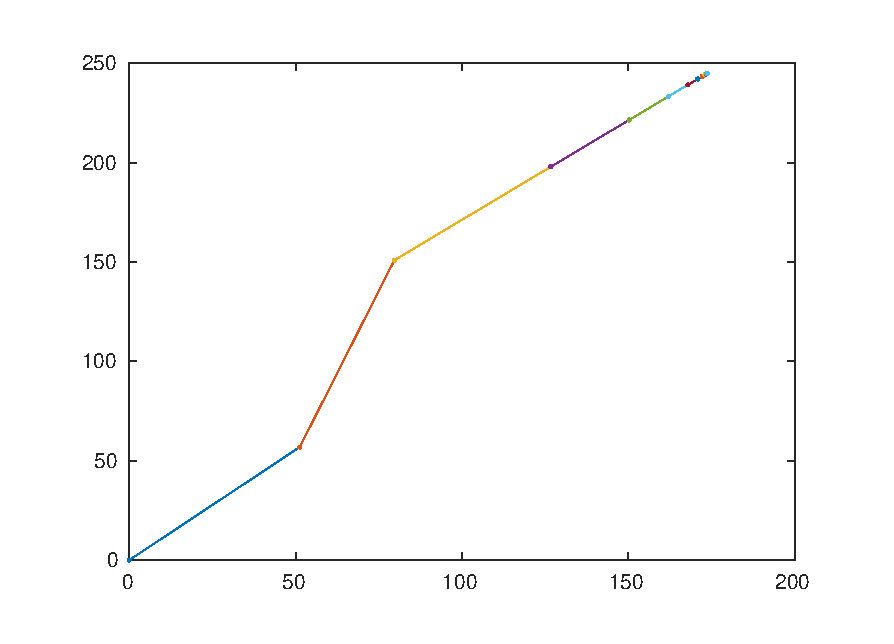
\includegraphics[width=.8\textwidth]{gaussSeidel1.eps}
\end{figure}

\item The Gauss-Seidel method gives $[173.7931, 245.0580, 253.7671]^T$
after 6 iterations. The first two coordinates at each iteration are
displayed below:

\begin{figure}[h!]
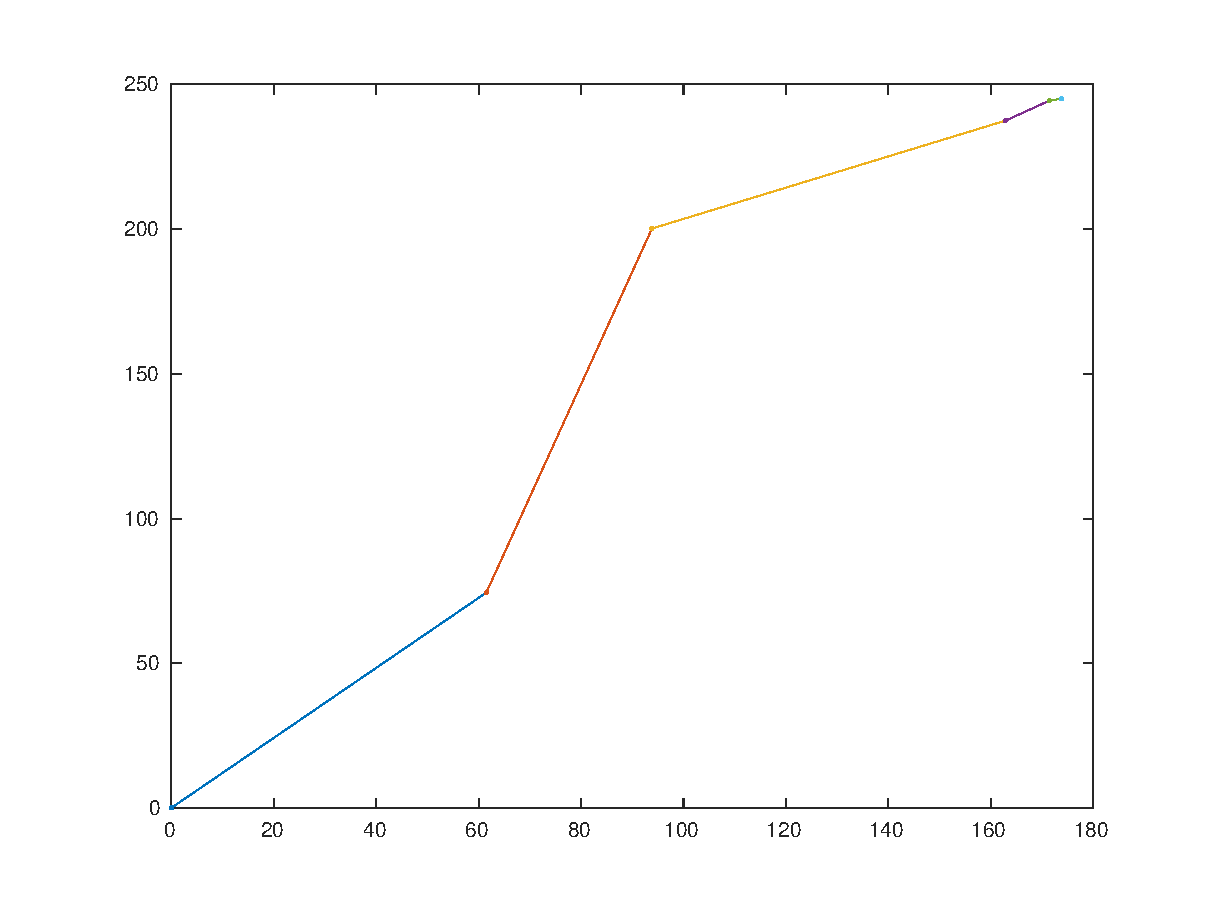
\includegraphics[width=.8\textwidth]{gaussSeidel2.eps}
\end{figure}

\end{enumerate}

\vfill
\pagebreak


\item Consider a matrix $F$ which acts on a vector in
$\RR^2$ by mapping $(x_1,x_2)$ to $(x_2, x_1 + x_2)$.

\begin{enumerate}
\item Write $F$ down explicitly.

\vspace{5mm}

The matrix sends $(1,0)$ to $(0,1)$ and $(0,1)$ to $(1,1)$;
therefore, the corresponding linear transformation is:

\[ F = \left[ \begin{array}{cc} 0 & 1 \\ 1 & 1
\end{array} \right] \]

\item Let $v = [0,1]$. In a $2 \times 11$ matrix, 
display $F^kv$ for $k = 0, 10$.

\vspace{5mm}


We use the following MATLAB code to carry out this operation:
\begin{verbatim}
F = [0 1; 1 1];
v = [0 1]';

M = zeros(2,11);
for i=0:10
    M(:,i+1) = F^i*v;
end
\end{verbatim}

\vspace{5mm}

The computed matrix is:

\begin{verbatim}
M =

     0     1     1     2     3     5     8    13    21    34    55
     1     1     2     3     5     8    13    21    34    55    89
\end{verbatim}

The top row is the Fibonacci sequence, and the bottom row is the
same sequence shifted by $1$.

\item What are the eigenvalues and eigenvectors of $F$?
Use this to write an explicit formula for $F^k$.

\vspace{5mm}

To compute the eigenvalues and eigenvectors, we can use
the polynomial method:

\[  \left|\begin{array}{cc} \lambda & -1 \\ -1 & \lambda-1
\end{array} \right| = \lambda^2 - \lambda - 1 = 0 \hspace{5mm}
 \Rightarrow \lambda = \frac{1 \pm \sqrt{5}}{2} \]

For convenience, denote the roots by $\lambda_+$ and $\lambda_-$. 
The corresponding eigenvectors can be derived using the following equations:

\[  \left(\begin{array}{cc} \lambda_+  & -1 \\ 
-1 & \lambda_+ - 1 \end{array} \right) 
\left( \begin{array}{c} x_1 \\ x_2 \end{array} \right) = 0    \hspace{5mm}
 \Rightarrow x_2 = \lambda_+ x_1 \]
\[  \left(\begin{array}{cc} \lambda_-  & -1 \\ 
-1 & \lambda_- - 1 \end{array} \right) 
\left( \begin{array}{c} x_1 \\ x_2 \end{array} \right) = 0    \hspace{5mm}
 \Rightarrow x_2 = \lambda_- x_1 \]

The corresponding eigenvectors are thus $v_+ = [1, \lambda_+]^T$ and 
$v_- = [1, \lambda_-]^T$. Using this formulation, the change-of-basis matrix
\[ P = \left[ \begin{array}{cc} 1 & 1 \\ \lambda_+ 
& \lambda_- \end{array} \right], \hspace{1cm} 
P^{-1} =  \frac{-1}{\sqrt{5}}
\left[ \begin{array}{cc} \lambda_- & -1 \\ 
- \lambda_+ & 1  \end{array} \right].\]

Using these formulae for $P$ and $P^{-1}$,
\[F^k = P \left[ \begin{array}{cc} \lambda_+^k & 0 \\ 
0 & \lambda_-^k \end{array} \right] P^{-1}.\]


\item Use everything you have done so far to write a formula
for the $k$-th Fibonacci number, where $F_0 = 0$ and $F_1 = 1$.

\vspace{5mm}

As we saw before, the first coordinate of $F^kv$ 
for $v = [0,1]^T$ is the $k$-th Fibonacci number. 
The formula for this, based on the last answer, is:

\[  \text{ first entry of   } \left[ \begin{array}{cc} 1 & 1 \\ \lambda_+ 
& \lambda_- \end{array} \right]
\left[ \begin{array}{cc} \lambda_+^k & 0 \\ 0 & \lambda_-^k \end{array} \right]\frac{-1}{\sqrt{5}}
\left[ \begin{array}{cc} \lambda_- & -1 \\ 
- \lambda_+ & 1  \end{array} \right] \left[ \begin{array}{c} 0 \\ 1 \end{array} \right]. \]
\[ =  \text{ first entry of   }
\left[ \begin{array}{cc} 1 & 1 \\ \lambda_+ 
& \lambda_- \end{array} \right]  \left[ \begin{array}{cc} \lambda_+^k & 0 \\ 0 & \lambda_-^k \end{array} \right] \left[ \begin{array}{c} 1/\sqrt{5} \\ -1 / \sqrt{5} \end{array} \right] \]
\[ =  \left[ \begin{array}{cc} 1 & 1 \end{array} \right] \left[ \begin{array}{c} \lambda_+^k/\sqrt{5} \\ - \lambda_-^k/ \sqrt{5} \end{array} \right] = \dfrac{\lambda_+^k - \lambda_-^k}{\sqrt{5}} \]

To summarize, $F_k = \dfrac{
\left( \dfrac{1 + \sqrt{5}}{2} \right)^k - 
\left( \dfrac{1 - \sqrt{5}}{2} \right)^k}{\sqrt{5}}$.\\
For $k \geq 2$, the power of $\lambda_-$ is less than $1/2$,
so it is sufficient to take the integer closest to the first term.
\end{enumerate}
\end{enumerate}

\end{document}
